\documentclass{article}

\usepackage{tikz}
\usepackage{circuitikz}
\usepackage[utf8]{inputenc}
\usepackage[english,bulgarian]{babel}
\usepackage{graphicx}
\usepackage{caption}
\usepackage{amsmath}
\usepackage{float}
\numberwithin{equation}{section}


\title{Приложение на математиката за моделиране на реални процеси. Моделиране на неврон.}
\author{Тонка Желева \and Васил Пашов}

\begin{document}

\maketitle
\newpage

\tableofcontents
\newpage

\section{Науката за невроните и приложение}

Мозъкът, намиращ се в черепната кухина, е част от централната нервна система. Той е основният орган, който обработва всички съзнателни и
несъзнателни стимули, чувства,  познания и памет. Също така е отговорен за контролирането на множество други органи. Основната градивна
единица на мозъка е невронът. Човешкият мозък съдържа около $10^{11}$ неврона. Нервните клетки приемат, обработват и изпращат нервния импулс.

Животните реагират на външни въздействия, използвайки невроните.  Например, при заплаха от изгаряне, рецепторите за топлина на сензорен
неврон осъществяват връзка със стимула и изпращат информация до интер-неврон в централната нервна система. Оттам мото-неврон изпраща
отговора до скелетните мускули, които карат тялото да се отдръпне. В основата на извършването на този процес стои невротрансмисията, която
се извършва във всички неврони в човешкото тяло. Невроните пренасят тази информация чрез промени в електрическия потенциал на мембраната.

Науката, която се занимава с изследването на нервната система, е изключително обширна. Тя се разделя на много дялове, като те обващат
най-различни аспекти -- от изучаването на невроните на клетъчно ниво, психология, клинична част, занимаваща се със заболявания на нервната
система, до приложения на невронните мрежи, чрез които се симулират реални процеси чрез компютри и много други.

В последните десетилетия чрез науката за невроните хората успяват да изучат много болести, като също така предоставят адекватно лечение или
подобрение при пациентите, въпреки това някои процеси остават загадка и предизвикателство, което да бъде разрешено вбъдеще. Пример за
заболяване, пряко свързано с протичането на нервните импулси, е множествената склероза. Множествената склероза (MC) засяга способността на
нервните клетки на главния и гръбначния мозък да комуникират помежду си. Аксоните са обгърнати от изолираща субстанция – миелин. При МС
собствената имунна система атакува и унищожава миелиновото покритие. Когато миелинът бъде загубен, аксоните не могат да провеждат ефективно
сигналите. Въпреки обширните познания за протичането и прогресирането на заболяването, пусковият механизъм остава засега неизвестен. Не
съществува познато лекарство за множествена склероза. Лечението е насочено към възстановяване на функциите след пристъп, превенция от нови
пристъпи и предотвратяване на трайната инвалидизация.

\section{Устройство на неврона}
За да можем моделираме протичането на нервния импулс, трябва да се запознаем с устройството на неврона и да разберем какви процеси протичат в него. Накратко ще разгледаме основните части, изграждащи нерврона и осъществяващи преноса на сигнали.

\begin{figure}[H]
    \centering
    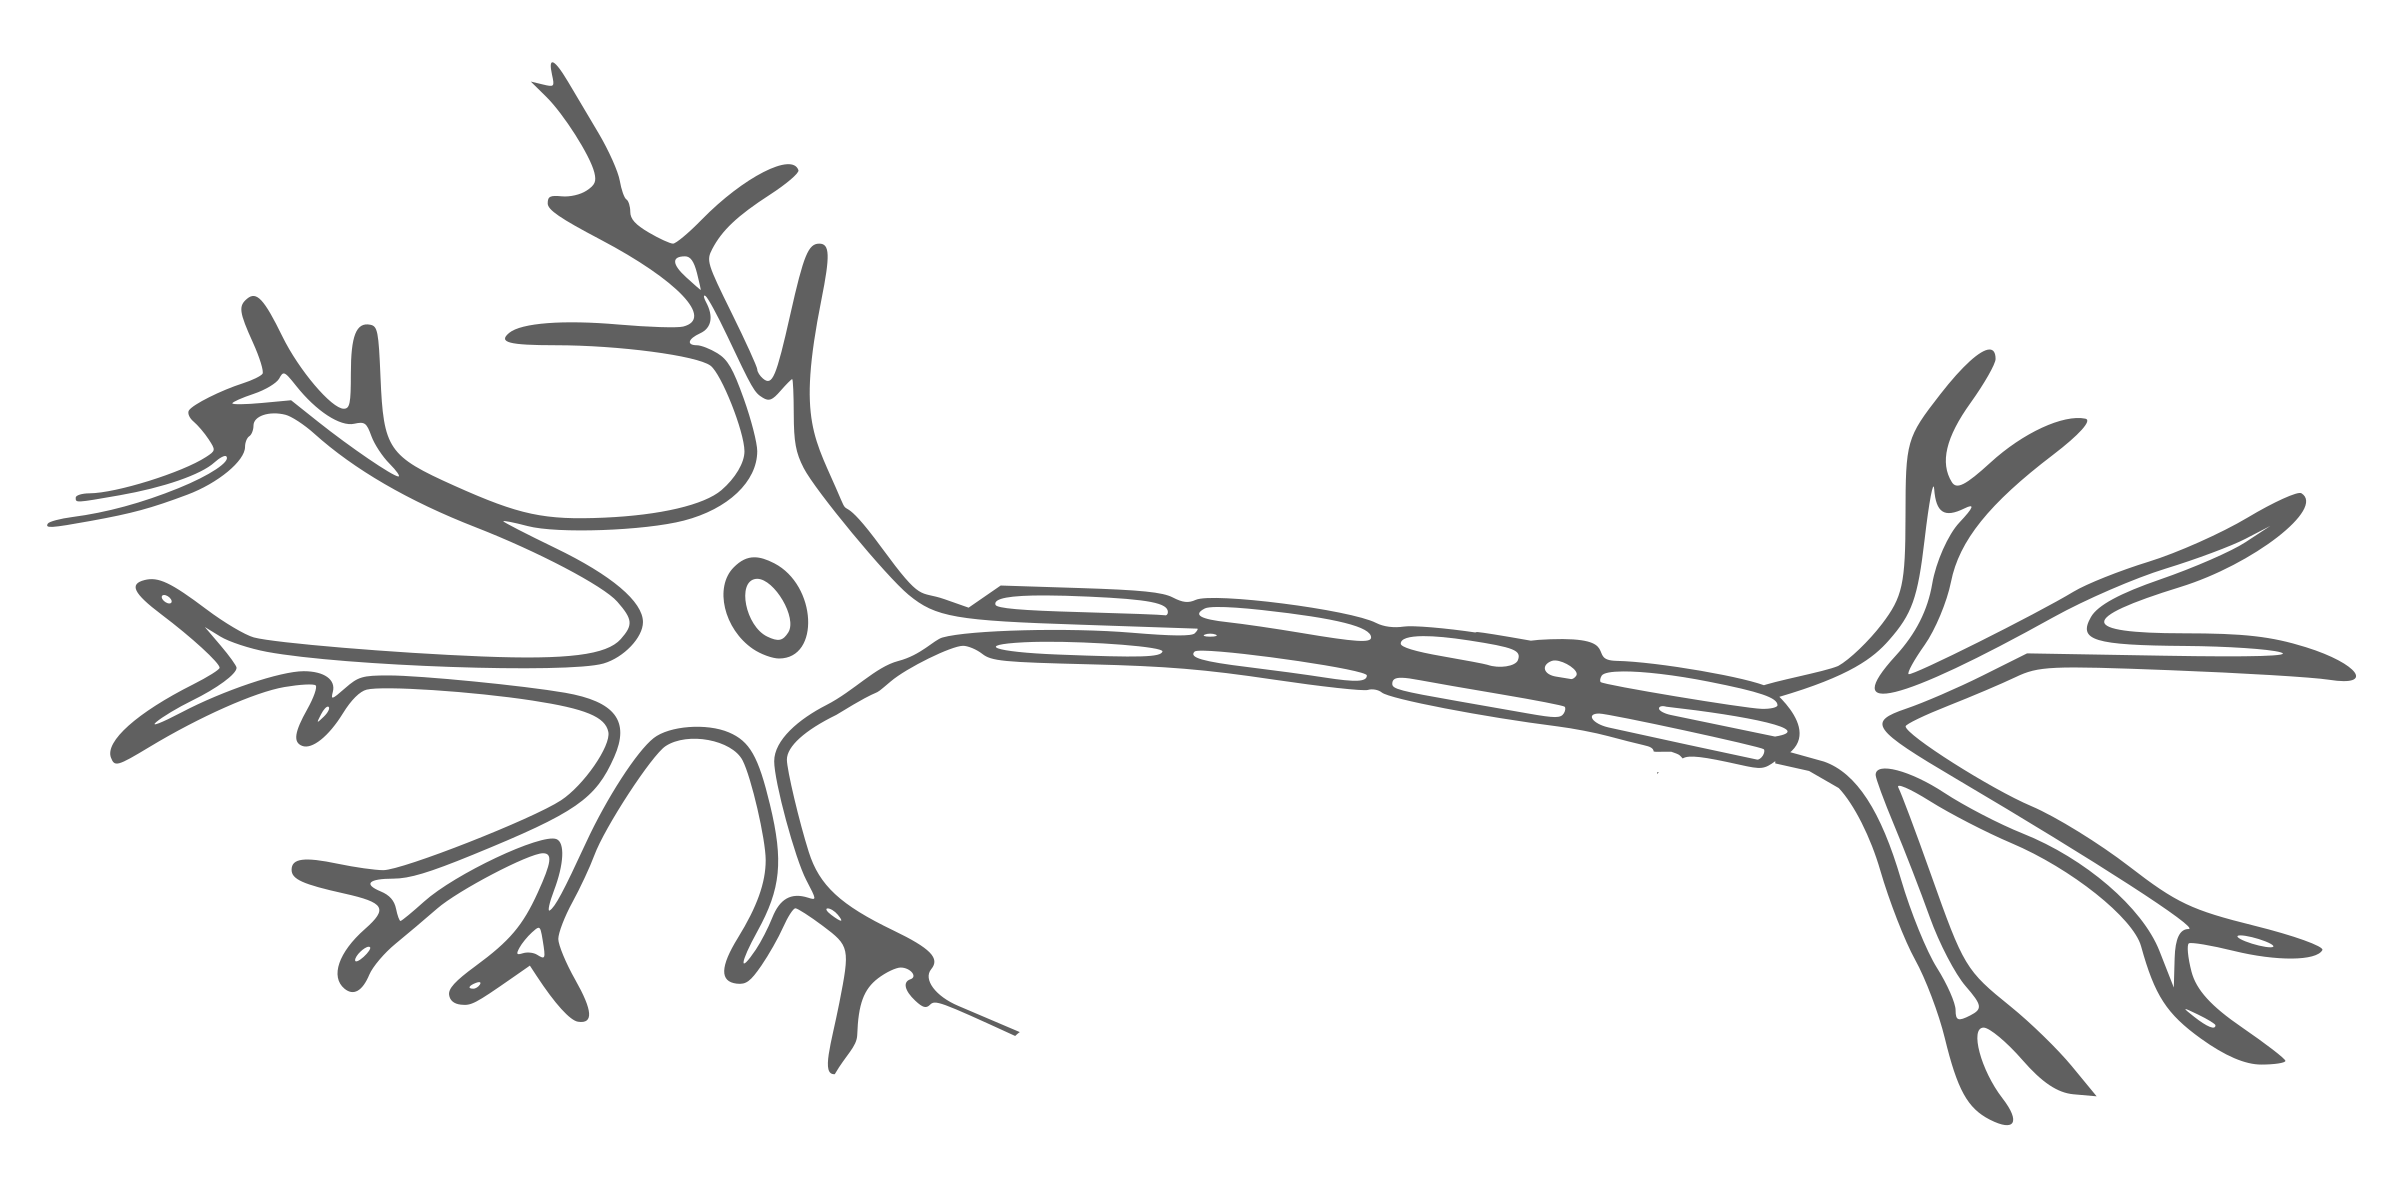
\includegraphics[scale=0.5]{./schemas/Neurona.png}
    \caption{Неврон}
\end{figure}

\textbf{аксон} -- най-издълженият израстък на неврона, чиято дължина може да надхвърли десетки хиляди пъти диаметъра на клетъчното тяло. Аксонът
извежда нервните импулси от клетъчното тяло, пренасяйки информация до друга клетка. Нервните импулси са еднопосочни , но неврона
може да получи информация под формата на протеини, които се придвижват от синапса до клетъчното ядро. В своя край аксонът се разклонява в
образувания, наречени терминали. Тези акосанални терминали осъществяват връзката с клетките, които трябва да получат сигнала.  Много неврони
имат само един аксон, но той се разклонява в много направления и така прави възможна комуникацията с много клетки.

\textbf{дендритни дървета} -- изградени от разклонени израстъци на нервната клетка. Повечето неврони получават сигнали през своите дентритни
дървета. Един неврон може да има повече от една група дендрити, чрез които получава хиляди сигнали.

\textbf{клетъчна мембрана} -- плазмената мембрана е изградена от двоен липиден слой. В него са вградени мембранни белтъци, които изпълняват
важни функции: транспортни, енергетични, структурни, сензорни. Строежът, съставът и формата на една мембрана не са постоянни, а динамично се
изменят според функциите, които трябва да извършва и според състоянието на клетката.

\textbf{синапси} -- специфични структури, осъществящи провеждането на нервния импулс. За целите на нашата задача ще разгледаме химическия
синапс. Химическият синапс е специално съединение между два неврона, което позволява те да си комуникират без да са физически свързани.

\section{Моделиране на електрическите свойства на клетъчната мембрана} Тъй като електрическите сигнали са в основната на преноса на
информация в нервната система, е необходимо да разберем как се пораждат и пренасят тези сигнали. Проблем при невроните представляват
акосните, тъй като те са дълги и не са добри проводници. За да се компенсира този недостатък, невроните развиват система, която им помага да
пренасят сигнали на голямо разтояние, въпреки техните лоши електрически характеристики.  Електрическите сигнали, възпроизведени от тази
система, се наричат акционни потенциали или импулси. Ключова роля в тази система заема клетъчната мембрана.

Всички животински клетки са обградени от мембрана, състояща се от двоен липиден слой, в който са вградени протеини. Мембраната служи както
за изолатор, така и за дифузионна бариера за движението на йоните. Транспортни протеини (помпи) изтласкват навън йони, а йонните каналчета
позволяват на йоните да прекосят мембраната и да навлязат в клетката.

\vspace{5mm} %5mm vertical space
\textbf{Видове йони, намиращи се в клетката}

В невроните и обграждащата ги течност най-често срещани са следните йони:
\begin{itemize}
  \item положително заредени -- натриеви и калиеви,
  \item отрицателно заредени -- хлорни.
\end{itemize}

В повечето неврони К+ йони са с по-голяма концентрация във вътрешността на клетката. Обратно, обикновено Na+ и Cl- са с по-голяма концентрация извън клетката

\vspace{5mm}
\textbf{Как йоните преминават през мембраната}

Тъй като са заредени, йоните не могат да преминат директно през хидрофобните липидни области на мембраната. Вместо това те трябва да
използват специализираните протеини, които образуват хидрофилен тунел през мембраната. Някои от каналчетата са отворени, когато невронът е в
покой, а други се активирит при въздействие от сигнал. Някои йонни каналчета имат избирателна пропускливост спрямо различните видове
йони, съответно се наричат калиеви и натриеви каналчета.

\vspace{5mm} %5mm vertical space

Мембранният потенциал се дефинира като разликата между потенциалите във вътрешността на клетката и извънклетъчната среда.
Понеже има разлика в потенциалите в клетъчната мембрана, казваме, че мембраната е поляризирана:
\begin{itemize}
  \item aко мембранният потенциал стане по-голям от равновесния потенциал, казваме, че мембраната е дополяризирана;
  \item aко мембранният потенциал стане по-малък от равновесния потенциал, казваме, че мембраната е хиперполяризирана.
\end{itemize}

Всички електрически сигнали, които използват невроните за комуникация, представляват деполяризация или хиперполяризация на равновесния мемранен потенциал.

\vspace{5mm} %5mm vertical space
\textbf{Равновесен мембранен потенциал}
Равновесният потенциал се определя от неравното разпределение на йони между вътрешността и външната среда на клетката и различната пропускливост на клетката към различните видове йони.


\vspace{5mm} %5mm vertical space
\subsection{Процесът на невротрансмисия и акционният потенциал}
В нервната клетка навлизат два вида сигнали, които могат да бъдат стимулиращи, които възбуждат неврона, т.е. генерират електрически импулс,
или инхибиращи - предотвратят неврона от активиране.  Дали един неврон ще е активиран зависи от сумата на възбуждащите и възпиращите
сигнали.  Връзката между два неврона се осъществява чрез синапси. В повечето синапси информацията се предава чрез химически съобщения,
наречени невротрансмитери. Когато акционният потенциал преминава по аксона и достига аксонния терминал, той отключва освобождаването на
невротрансмитер в синаптичната цепнатина.

Невротрансмитърите прекосяват синапса и се смесват с мембранните рецептори на постсинаптичната клетка, предавайки стимулиращия или инхибиращ
сигнал. Невронът завършва с малко разширение, наречено присинаптичен терминал. От другата страна на неврона имаме постсинаптичен терминал.
Акционният потенциал кара калциевите йонни каналчета на терминала да се отворят. Невротрансмитерите се освобождават чрез екзоцитоза. Те
бързо дифузират в синаптичната празнина. Когато достатъчно калиеви каналчета се отворят, постсинаптичната празнина се деполяризира и
акционният потенциал продължава по неврона. Това води до деполяризация (смяна на поляритета) -- отвътре клетката се зарежда положително.
Следва реполяризация и се получава акционен потенциал. Промените в мембраната  са израз на възбуждане и се наричат възбуждащ постсинаптичен
потенциал. Големината на постсинаптичния потенциал зависи от количеството на отделения медиатор и от чувствителността на постсинаптичната
мембрана.

\vspace{5mm} %5mm vertical space
\textbf{Акционен потенциал}

Когато входен сигнал достигне тялото на клетката, невронът ще ускори разпространяваща се промяна в мембранния потенциал. Преминаващата вълна
на електричество се нарича акционен потенциал. Акционните потенциали преминават с константна скорост от около 100m/s и с константна честота.
В спокойно състояние невроните имат равновесен потенциал от -60 до -70 mV. Това означава, че вътрешната част на клетката е отрицателно
заредена.

\vspace{5mm} %5mm vertical space
\textbf{Цикъл на акционния потенциал}

\begin{itemize}
\item Акциноният потенциал се задейства, когато деполяризацията увеличи мембранното напрежение, така че де премине граничната стойност, която е
обикновено -55mV.
\item При достигането на тази граница, Nа+ каналчета, зависещи от напрежението, се отварят и позволяват на натриевите йони да
навлязат в клетката. Този поток от натриеви йони увеличава мембранния потенциал много бързо, докато той достигне +40mV.
\item След кратък период от време, натриевите каналчета се самодеактивират, спирайки навлизането на натрия.
\item Множество калиеви каналчета, зависещи от напрежението, се отварят, позволявайки на калия да излезе извън клетката. Това бързо намалява
    мембранния потенциал, връщайки го обратно в нормалното му равновесно положение. Калиевите каналчета остават отворени по-дълго време, но
    в крайна сметка те се затварят и мембранни потенциал се стабилизира.
\item Натриевите каналчета се връщат в нормалното си състояние, затворени, но очакващи стимулиращо напрежение.  Така цикълът на акционния
потенциал може да започне отново.
\end{itemize}
\vspace{5mm} %5mm vertical space
\textbf{Предаване на сигнала от акционния потенциал}

Потенциалът на аксона може да преминава само в една посока -- от тялото на клетката към терминала на аксона. Когато една област от
мембраната e подложена на въздействието на акционния потенциал, много Nа+ йони, навлизат в тази част на клетката. Тези йони се разпръскват
във вътрешността на клетката и могат да деполяризират съседни области на мембраната, подтиквайки отварянето на натриевите каналчета и
предизвиквайки протичането на акционен потенциал в тази част.

\vspace{5mm} %5mm vertical space
\subsection{Мембраната като електрическа верига}

За да можем да моделираме електрическите свойства на мембраната, ще ги представим като елементи в еквивалентната \'{и} електрическа схема.
Хидрофилните участатъци на молекулите, изграждащи клетъчната мембрана, притежават способността да се йонизират, а хидрофобните участаци
образуват централен диелектричен слой. Така можем да определим клетъчната мембрана като кондензатор, който се характеризира с електричен
капацитет. Капацитетът на един кондензатор, $c$, расте с увеличаване на площта на плочите, $A$, и намалява с увеличаване на разстоянието
между тях, $d$. В биологичните мембрани дебелината на хидрофобния участък от липидния бислой е много малка – около 2.5 nm. Това определя
много висока стойност на мембранния капацитет – близо до 1 $\mu F/cm^2$ .  Използваме следната формула за изчисляване на “специфичния
капацитет”: $C_{m}=\frac{c}{A}=\frac{\epsilon}{d}$. Натрупването на заряд от двете страни на мембраната, получен от разликата в
концентрацията на йоните, предизвиква потенциална разлика между вътрешната и външната част на клетката. Тя може да бъде измерена с формулата
$Q=CV$. Тъй като капацитетът на мембраната е голям, дори натруDпването на малък заряд от двете \'{и} страни води до голяма потенциална
разлика. 

\vspace{5mm} %5mm vertical space
\textbf{Йонни токове, протичащи през мембраната}

Всеки йоннен ток се характеризира с две компоненти -- кодуктивен ток, зависещ от разликата в напреженито на мембраната, и дифузионен ток,
зависещ от разликата в концентрацията на йоните. Електричното поле, което се създава от капацитета на мембраната, упражнява сила върху
електрическите заряди на йоните и ги кара да се движат, това се нарича кондуктивен ток. Плътността на кондуктивния ток се определя със
следното уравнение $J_c=\tilde{G}_{Na}V$, където $\tilde{G}_{Na}$ е проводимостта на натрия за определена мярка площ. Дифузионният се
определя от разликата в концентрацията на йоните. Плътността на дифузионният ток може да се изрази с уравнението
$J_d=-qD_{Na}\frac{d[Na+]}{dx}$, където $D_{Na}$ e дифузионната константа за натриевите йони. Имаме знак минус, защото йоните дифузират в
посока, обратна на тази, където концентрацията им е по-голяма. Формулите, които използваме за натриевите йони са аналогични за другите йони.
Кондуктивният ток може да стане равен на 0, когато разликата в напрежението на мемраната е 0, а дифузионният ток може да стане равен на 0,
когато концентрацията на йоните от двете страни на мембраната се изравнят. 

От релацията на Айнщайн (свързваща дифузионната констанстанта с хаотичното движение на частици, породено от сблъсъка им с хаотично движещите
се водни молекули) и температурното равновесие имаме следния извод: $J_c + J_d = 0$.

Използвайки формулата за капацитивни ток $J_{cap}=C\frac{dV}{dt}$ и горните две формули за кондуктивния и дифузионен ток, общият йонен ток, протичащ през мембраната, можем да изразим така:

\begin{equation}\label{trans_memb_curr}
        J = C\frac{dV}{dt} + J_{Na} + J_{K} + J_{Ca} + ...
    \end{equation}

\vspace{5mm} %5mm vertical space
\textbf{Йонни проницаемости}

Експериментално Ходкин и Хъксли са установили, че най - голямо влияние в уравнение \eqref{trans_memb_curr} имат натрия и калия. Освен това
са достигнали до модел описващ вероятността, съответните канали да се отворят или затворят. При калиевите йони тази вероятност зависи само
от константа за активация на калиевия канал - $m$, докато при натриевите йони, освен константа за активация - $n$ имаме и константа за
деактивация - $h$. Констаните за активация съответно зависят от скоростни константи $\alpha$ и $\beta$, по следния начин:

\begin{equation}\label{chanels}
    \begin{aligned}
        &\frac{dm}{dt} = \alpha_m(1-m) - \beta_mm\\
        &\frac{dh}{dt} = \alpha_m(1-h) - \beta_hh\\
        &\frac{dn}{dt} = \alpha_m(1-n) - \beta_nn\\
    \end{aligned}
\end{equation}

Нека с $\bar{J_{Na}}$ и $\bar{J_{K}}$, означим съответно максималната пропускливост на натриевите и калиевите канали. Тогава
уравнение \eqref{trans_memb_curr} придобива следния вид:

\begin{equation}\label{trans_memb_curr_h-h}
    J = C\frac{dV}{dt} + J_{Na}mh^3 + J_{K}n^4 + J_{L}
\end{equation}

Където $J_{L}$ е малък поток, представляващ собра на останалите членове от \eqref{trans_memb_curr}

\section{Модел на Ходжкин-Хъксли}
    \subsection[Експериментални методи]{Експериментални методи}
        За да можем да изследваме напълно някое свойство на даден предмет, трябва да можем да го контролираме процесите, в които това
        свойство се проявява.  Един от най - важните ппроцеси за нас е процесът по обмяна на вещества.  Обмяната на вещества от своя страна,
        обаче влияе на напрежението в неврона, което от своя страна влияе на обмяната на веществана. Виждаме, че се получава цикличен
        процес, който се изследва много трудно. За наше щастие съществува начин, по който да фиксираме напрежението в неврона. Този метод са
        използвали Ходжкин и Хъксли. Нека разгледаме следната схема:

        \begin{figure}[H]
            \centering
            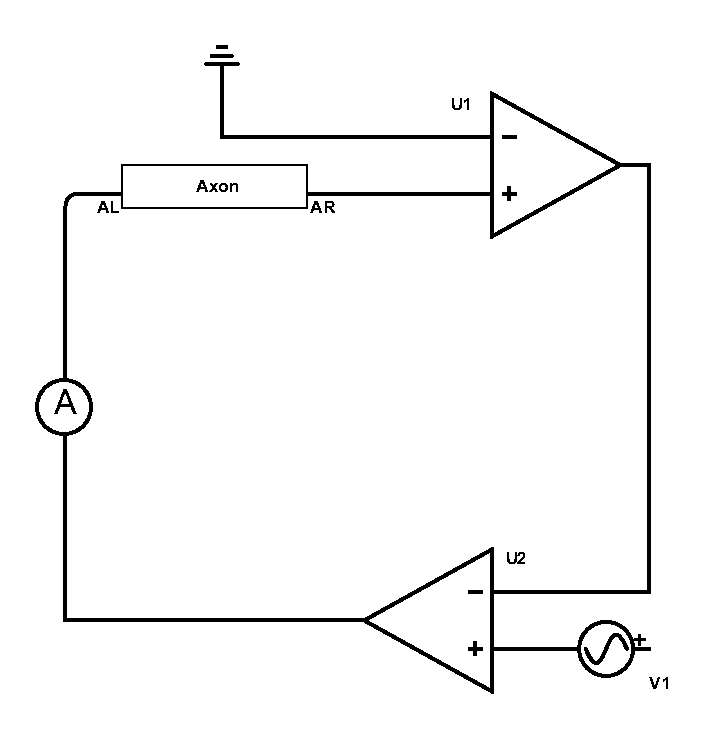
\includegraphics[scale=0.6]{./schemas/voltage-clamp.pdf}
            \caption{Електрическа схема за фиксиране на напрежението}
        \end{figure}

        През аксона е прокаран дълъг и тънък проводник, свързан с положителния вход на усилвател с коефициент 1. Отрицателният вход на усилвателя
        е заземен (или е свързан с течност като тази в която се намира неврона). По този начин усилвателя предава ток с напрежение $V_n$ равно на
        напрежението в самия неврон. Този ток се подава като отрицателен вход на друг усилвател с коефициент 1. На положителния вход на този
        усилвател се подава ток с напрежение двойно на желаното равновесно напрежение $V_d$. Този ток през амперметър и след това се подава в
        другия край на аксона. По този начин ако, $V_n > 2V_d$, в точката $AL$ напрежението ще бъде по - ниско от нормалното за акосна, за да се
        компенсира това положителните частици ще се насочат в тази посока, намаляки напрежението в аксона. Напрежението ще намалява клонейки към
        $V_n$ и, когато стане равно на $V_n$, токът, излизащ от усилвател $U_2$, ще бъде с напрежение $U_d$, като така се получава равновесие в
        системата.

        Ние разглеждаме неврона като дълъг и много тънък кабел. Както ще видим от модела, протичането на ток през неврона
        зависи от две променливи - време и пространство. Идеята на пространствената фиксация е да се изключи пространството.
        По този начин ако бъде предизвикан импулс, той ще се разпространи по целия аксон едновременно. Това се постига като
        през аксона се прокара дълъг и тънък проводник и неврона се постави в течност с ниско съпротивление.
    \subsection{Извеждане на математическия модел}
    Ще разглеждаме невронa като дългъг и тънък кабел. Това означава, че напрежението/токa, по него ще зависи само от една пространствена
    променлива -- $x$. Нека с $i\left(x, t\right)$ означим трансмембранния ток $x$, в момента $t$, a с $j\left(x, t\right)$ означим потока на електрически заряди в точка $x$. С други думи, $j\left(x, t\right)$ e
    скоростта, с която преминава електрическя заряд през точката, $x$. Нека сега разгледаме един, достатъчно малък интервал от неврона
    $\left[\xi, \xi+\Delta\xi\right]$:

    \begin{figure}[H]
        %Uncomment next line if XeTeX is used
%\def\pgfsysdriver{pgfsys-xetex.def}
\baselineskip=10pt
\hsize=6.3truein
\vsize=8.7truein
\tikzpicture[line cap=round,line join=round,>=triangle 45,x=1.0cm,y=1.0cm,scale=0.7]
\clip(-1,-5.04) rectangle (19.62,6.3);
\draw (2,-2)-- (14,-2);
\draw (2,2)-- (14,2);
\draw (6,2)-- (6,-2);
\draw (10,2)-- (10,-2);
\draw [->] (2,0) -- (6,0);
\draw [->] (10,0) -- (14,0);
\draw [->] (8,0) -- (8,4);
\fill [color=black] (6,-2) circle (1.5pt);
\draw[color=black] (5.96,-2.28) node {$\xi$};
\fill [color=black] (10,-2) circle (1.5pt);
\draw[color=black] (10.7,-2.28) node {$\xi+\Delta\xi$};
\draw[color=black] (4.32,0.22) node {j($\xi$,t)};
\draw[color=black] (12.5,0.24) node {j($\xi+\Delta\xi$,t)};
\draw[color=black] (8.82,2.72) node {i(x,t)};
\endtikzpicture


        \caption{}
    \end{figure}

    Токът във всяка една точка в интервала е равен на разликата във входящия ток и изходящия ток, това води до следното уравнение:
    \begin{equation}\label{integral_form}
        j\left(\xi,t\right) - j\left(\xi + \Delta\xi, t\right) = \int_{\xi}^{\xi + \Delta\xi} i\left(x,t\right)dx
    \end{equation}

Уравeние \eqref{integral_form} представлява закона за запазване в интегралната му форма. Ние сега ще го приведем в диференциална форма.
Първо апроксимираме интеграла в дясната част, използвайки формулата на правоъгълниците, и получаваме:

    \begin{gather*} 
        j\left(\xi,t\right) - j\left(\xi + \Delta\xi, t\right) = i\left(\xi + \frac{\Delta\xi}{2},t\right)\Delta\xi +
        O\left(\Delta\xi^3\right)\\
     \end{gather*}

    Сега делим на $\Delta\xi$ и пускаме $\Delta\xi$ да клони към 0 и получаваме следното за тока през аксона:
     
    \begin{gather*} 
        \frac{j\left(\xi,t\right) - j\left(\xi + \Delta\xi, t\right)}{\Delta\xi} = i\left(\xi + \frac{\Delta\xi}{2},t\right) +
        O\left(\Delta\xi^2\right)\\
        i\left(\xi,t\right) = -\frac{dj}{dx}\left(\xi,t\right)
     \end{gather*}

     От закона на Ом знаем, че $I = \frac{U}{R}$, а експериментално е установено, че $j(x,t) = \frac{di}{dx}$. Като заместим получаваме:

     \begin{equation}
         i(\xi,t) = \frac{1}{R}\frac{d^2V(\xi,t)}{dx^2}
     \end{equation}

     Сега изразяваме $i$ от \eqref{trans_memb_curr_h-h}, като с $j_{ion}$ означаваме йонния поток.

     \begin{equation}
        \begin{aligned}
            &\frac{dV}{dt} = \frac{1}{R}\frac{d^2V}{dx^2} - \frac{j_{ion}}{c}\\
            &\frac{dm}{dt} = \alpha_m(1-m) - \beta_mm\\
            &\frac{dh}{dt} = \alpha_m(1-h) - \beta_hh\\
            &\frac{dn}{dt} = \alpha_m(1-n) - \beta_nn\\
        \end{aligned}
     \end{equation}

    \subsection{Апроксимация на модела} 
    Получената система от диференциални уравнения е изключително трудна за решаване. Затова ще я апроксимираме с числен метод. За тази цел
    трябва да дискретизираме областта, в която търсим решенията, както въведем равномерна мрежа от възли. В тези възли ще търсим
    приближеното решнение. След това ще апроксимираме прозиводните. Нека с $h$, $\tau$ и $y_i^j$ означим съответно стъпката по
    пространството, времето и приближеното решение в точка $x_i$ и момент $t_j$. 
    
    Апроксимираме $\frac{\partial^2 V}{\partial x^2}$ с формулата за апроксимация на производни от втори ред и получаваме:

    \begin{equation}\label{der:mid_space}
        \frac{\partial^2 V}{\partial x^2} \approx \frac{y_{i-1}^j - 2y_i^j + y_{i+1}^j}{h^2}
    \end{equation}
    
    Апроксимираме производната по времето $\frac{\partial V}{\partial t}$ с формулата за разлика напред и получаваме:

    \begin{equation}\label{der:forward_time}
        \frac{\partial V}{\partial t} \approx \frac{y_i^{j+1} - y_i^j}{\tau}
    \end{equation}

    Аналогично на \eqref{der:forward_time} апроксимираме и прозиводните: $\frac{dm}{dt}, \frac{dn}{dt}, \frac{dh}{dt}$

    Замествайки тези резултати в системата получаваме следната апроксимация на модела на Ходжкин-Хъксли изразено спрямо неизвестното
    $y_i^{j+1}$.

    \begin{equation}\label{approx:H-H}
        \begin{aligned}
            &y_i^{j+1} = \frac{\tau}{rch^2}\left(y_i^j +y_{i+1}^j\right) + y_i^j\left(1 - 2\frac{\tau}{h^2}\right)\frac{1}{rc}
            - \frac{j_{ion}}{c}\tau\\
            &m_i^{j+1} = \left(\alpha_m(1-m) - \beta_mm\right)\tau + m_i^j\\
            &h_i^{j+1} = \left(\alpha_h(1-h) - \beta_hh\right)\tau + h_i^j\\
            &n_i^{j+1} = \left(\alpha_n(1-n) - \beta_nn\right)\tau + n_i^j
    \end{aligned}
    \end{equation}

    Системата \eqref{approx:H-H} ни дава триточков шаблон. След като са ни известни три от точките на един слой, можем да намерим една точка
    на следващия. Следващата фигура илюстрира това визуално, известни са ни точките на слой $j$, и чрез тях намираме точката слой $j+1$.
    \begin{figure}[h!]
        \begin{center}
        \baselineskip=10pt
\hsize=6.3truein
\vsize=8.7truein
\definecolor{fftttt}{rgb}{1,0.2,0.2}
\definecolor{qqffqq}{rgb}{0,1,0}
\definecolor{cqcqcq}{rgb}{0.75,0.75,0.75}
\tikzpicture[line cap=round,line join=round,>=triangle 45,x=1.0cm,y=1.0cm]
\draw [color=cqcqcq,dash pattern=on 1pt off 1pt, xstep=1.0cm,ystep=1.0cm] (-4.3,4.74) grid (2.66,6.3);
\clip(-4.3,4.74) rectangle (5.66,6.3);
\draw (-2,5)-- (-2,6);
\draw (-3,5)-- (-2,5);
\draw (-2,5)-- (-1,5);
\fill [color=black] (-4,5) circle (1.5pt);
\fill [color=qqffqq] (-3,5) circle (1.5pt);
\fill [color=qqffqq] (-2,5) circle (1.5pt);
\fill [color=qqffqq] (-1,5) circle (1.5pt);
\fill [color=black] (0,5) circle (1.5pt);
\fill [color=black] (1,5) circle (1.5pt);
\fill [color=black] (2,5) circle (1.5pt);
\draw[color=black] (2.26,5.12) node {j};
\fill [color=black] (-4,6) circle (1.5pt);
\fill [color=black] (-3,6) circle (1.5pt);
\fill [color=fftttt] (-2,6) circle (1.5pt);
\fill [color=black] (-1,6) circle (1.5pt);
\fill [color=black] (0,6) circle (1.5pt);
\fill [color=black] (1,6) circle (1.5pt);
\fill [color=black] (2,6) circle (1.5pt);
\draw[color=black] (2.38,6.1) node {j+1};
\endtikzpicture

        \caption{}
        \end{center}
    \end{figure}

    Очевидно е, че този шаблон не може да бъде поставен така, че да се открият първите и последните точки на всеки слой. Стойностите на тези
    точки са ни известни, обаче от граничните условия, а стойностите в първия слой са ни известни от началното условие.
\end{document} 
